\input{setup.tex}

% Режим шаблона (должен быть включен один из трех)
%\ВКРtrue
\Практикаtrue
%\Курсоваяtrue

\newcommand{\ГдеПроводитсяПрактика}{Юго-Западном государственном университете} % для практики
\newcommand{\РуководительПрактПредпр}{Куркина А. В.} % для практики
\newcommand{\ДолжнРуководительПрактПредпр}{директор} % для практики
\newcommand{\РуководительПрактУнивер}{Чаплыгин А. А.} % для практики
\newcommand{\ДолжнРуководительПрактУнивер}{к.т.н. доцент} % для практики
\newcommand{\Автор}{А. Р. Барыбиной}
\newcommand{\АвторРод}{Иванова И.И.}
\newcommand{\АвторПолностьюРод}{Барыбина Анастасия Руслановна} % для практики
\newcommand{\Шифр}{21-06-0163}
\newcommand{\Курс}{4 } % для практики
\newcommand{\Группа}{ПО-11б}


\begin{document}
\maketitle
\ifПрактика{}\else{
   \input{ЛистЗадания}
   \input{Реферат}}\fi
\tableofcontents
\input{Обозначения}
\ifПрактика{}\else{\input{Введение}}\fi
\section{Анализ предметной области}
\subsection{Принцип работы программно-информационной системы управления бизнесом}

Согласно федеральному закону «О применении контрольно-кассовой техники при осуществлении расчетов в Российской Федерации» практически все заведения общественного питания должны быть оборудованы кассовым аппаратом. Современные ККТ, при совершении расчетов, передают данные в налоговую службу, а также используют их для автоматизации бизнес процессов. Кассовая программа позволяет автоматизировать все рабочие процессы предприятия. Рассмотрим, основные из них:

\subsubsection{Обслуживание гостей}
После принятия заказа и внесения его в программу, он сразу же отправляется на кухонные и барные чековые принтеры. В чеках указывается название блюда, его количество, а также пожелания гостей касаемо их заказа. При расчете гость получает чек с перечнем заказанного, суммой оплаты, а также размером скидки, если она была используема. Помимо этого, кассовые программы упрощают управление системой лояльность. После проведения оплаты через кассу, данные передаются в налоговую службу.

\subsubsection{Кухня и бар}
Программно-информационные системы управления ресторанным бизнесом позволяют автоматизировать работу с технологическими картами, обеспечивая контроль не только за качеством приготовления пищи, но и использованием продуктов, ведения учёта остатков ингредиентов и готовых блюд. Более того, система сама подсчитывает количество калорий, белков, жиров и углеводов как в объеме приготовленного, так и для каждой порции.
Автоматизация процессов для бара также, как и для кухни, позволяет создавать и управлять техническими картами. Стоит отметить, что согласно Федеральному закону №171, при работе бара с алкогольными напитками система обязана передавать данные в ЕГАИС с помощью универсального транспортного модуля.


\subsubsection{Бухгалтерия}
Программы для оптимизации ресторанного бизнеса могу интегрироваться с сервисами для бухгалтерского учета, например, 1С или Контур.экстерн или Отчет.ру. Благодаря этому взаимодействию, накладные и данные о продажах автоматически отправляются бухгалтерам, за счет чего минимизируются ошибки и сокращается время ожидание документа. Главной целью, интеграции является оптимизация закупок, работы с поставщиками и расчета остатков.

\subsubsection{Управление прибылью}
Для управления прибылью в системе используется раздел «Аналитика», с помощью которого отслеживается эффективность работы сотрудников, производительность предприятия. Анализируются данные о продажах блюд, выручку, прибыль, рентабельность. На основе этой статистики, владельцы заведений общественного питания, могут изменять меню, проводить работы с сотрудниками, следить за развитием своего предприятия. 

\subsubsection{Сотрудники} 
Для удобства работы с сотрудниками, в системах автоматизации существует модуль управления работниками заведения. Он позволяет сохранять данные персонала в базу, отслеживать количество перерывов и выходных, отработанных часов и смен.


\subsection{Компоненты программно-информационной системы управления ресторанным бизнесом}
Программно-информационная система управления ресторанным бизнесом представляет собой комплекс взаимодействующих программ, аппаратных средств и методов, предназначенных для хранения, обработки и предоставления информации. Важным условием функционирования данной системы является наличие выделенной точки доступа WI-FI, которая обеспечивает взаимодействие между различными модулями. Для предотвращения несанкционированного доступа и обеспечения безопасности данных, сеть WI-FI должна быть защищена паролем и иметь свой уникальный идентификатор (SSID). 
На рисунке ~\ref{system:image} представлена схема взаимодействия программных продуктов, входящих в систему управления ресторанным бизнесом, а также способы их взаимодействия.

\begin{figure}[ht]
	\centering
	\includegraphics[width=1\linewidth]{system} 
	\caption{Схема взаимодействия компонентов системы управления ресторанным бизнесом}
	\label{system:image}
\end{figure}


\subsection{Кассовые отчёты}
Одной из причин использования кассовых программ в заведениях общественного питания является удобство формирования отчётов. В большинстве касс есть раздел "<Отчёты">, в котором представлена статистическая документация для таких категорий как касса, выручка, расход блюд, специальные отчёты. Рассмотрим обязательные отчёты: 

\subsubsection{Z-отчёт}
Буквой Z обозначается отчёт о закрытии смены. Он представляет собой документ, фиксирующий финансовые итоги деятельности кассовой техники за определенный период времени. Z-отчёт формирует данные денежных счетчиков на момент начала и окончания смены, данные об общей выручке до обнуления, сведения о предоставленных скидках, аннулированных чеках, а также информация о произведенных возвратах. Пример отчета представлен на рисунке ~\ref{zotchet:image}.

\begin{figure}[ht]
	\centering
	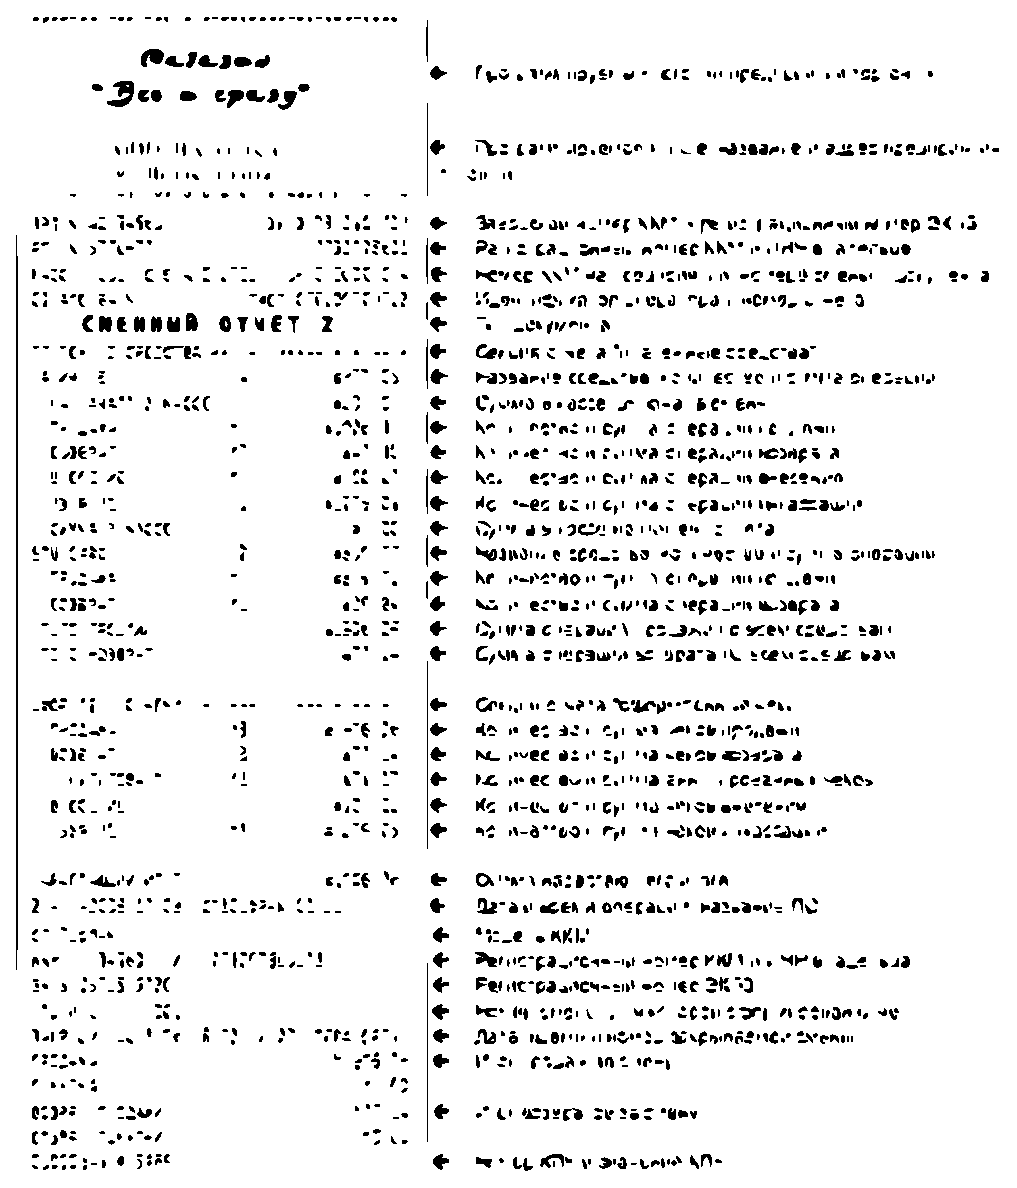
\includegraphics[width=0.7\linewidth]{zotchet} 
	\caption{Формат Z-отчёта}
	\label{zotchet:image}
\end{figure}

Ключевой особенностью данного отчёта является строго регламентированный временной интервал между двумя последовательными Z-отчётами, который не должен превышать 24 часа. Нарушение этого требования влечёт за собой блокировку кассового аппарата. Кроме того, каждому отчёту присваивается уникальный порядковый номер, исключающий возможность возникновения временных пробелов при формировании отчётности за определенный период времени.  

Поскольку в большинстве кассовых систем информация о закрытии смены фиксируется не только в контрольной ленте, но и в фискальной памяти устройства, Z-отчёт не подлежит обнулению и повторному формированию.  

В процессе обязательной регистрации контрольно-кассовой техники первоначальный Z-отчёт формируется и сохраняется в Инспекции Федеральной налоговой службы (ИФНС). Последующее формирование отчётов о закрытии смены приводит к обнулению оперативных данных о финансовой деятельности заведения за текущий день, а необходимые сведения автоматически передаются в налоговую. 

Z-отчёт необходим: 

\begin{itemize}
	\item кассиру для закрытия смены и передачи выручки в бухгалтерию: 
	\item бухгалтеру для контроля ежедневной выручки; 
	\item собственнику для анализа эффективности бизнеса; 
	\item сотрудникам налоговой для проверки правильности начисления и уплаты налогов. 
\end{itemize}

Содержание Z-отчёта должно соответствовать приказу ФНС России от 14.09.2020 № ЕД‑7‑20/662@. Перечень обязательных реквизитов представлена в Таблице \ref{zotchet:table}.

\begin{xltabular}{\textwidth}{|>{\raggedright\arraybackslash}p{5cm}|X|X|} 
	\caption{Обязательные данные для составления Z-отчёта\label{zotchet:table}} \\ \hline
	Наименование реквизита  & \centrow  Формат & \centrow Хранение \\ \hline
	\endfirsthead
	\continuecaption{Продолжение таблицы \ref{zotchet:table}}
	Наименование реквизита & \centrow Формат & \centrow Хранение \\ \hline 
	\finishhead
	Наименование документа& Печатный & - \\ \hline 
	Код формы ФД& Электронный & 5 лет \\ \hline
	Номер версии ФФД& Электронный &30 дней \\ \hline
	Наименование пользователя& Печатный & - \\ \hline
	ИНН пользователя & Печатный \newline Электронный & - \\ \hline
	Кассир& Печатный \newline Электронный & 30 дней \\ \hline 
	ИНН кассира& Печатный \newline Электронный & 30 дней \\ \hline
	Адрес расчётов& Печатный \newline Электронный & - \\ \hline
	Место расчётов& Печатный \newline Электронный & - \\ \hline
	Дата, время формирование документа& Печатный \newline Электронный & 5 лет \\ \hline
	Номер смены& Печатный \newline Электронный & 5 лет \\ \hline
	Регистрационный номер ККТ& Печатный \newline Электронный & 30 дней \\ \hline
	Количество кассовых чеков за смену& Печатный \newline Электронный & 30 дней \\ \hline
	Общее количество ФД за смену& Печатный \newline Электронный & 30 дней \\ \hline
	Количество непереданных ФД& Печатный \newline Электронный & 30 дней \\ \hline
	Дата первого непереданного ФД& Печатный \newline Электронный & 30 дней \\ \hline
	Признак превышения времени ожидания ответа ОФД& Печатный \newline Электронный & 30 дней \\ \hline
	Ресурс ключей фискального признака& Печатный \newline Электронный & 30 дней \\ \hline
	Номер фискального документа& Печатный \newline Электронный & 5 лет \\ \hline
	Номер фискального накопителя& Печатный \newline Электронный & 5 лет \\ \hline
	Фискальный признак документа& Печатный \newline Электронный & 5 лет \\ \hline
	Фискальный признак сообщения& Электронный & 30 дней \\ \hline
\end{xltabular} 
 
\subsubsection{X-отчёт}
Буквой X обозначают отчёт о текущем состоянии смен. Он представляет собой не фискальный документ, формируемый контрольно-кассовой техникой в течение открытой смены, так как информация, необходимая для формирования X-отчёта храниться в оперативной памяти ККТ и автоматически стирается, после закрытия смены.

В отличии от Z-отчёта X-отчёт не является документом строгой отчётности, передаваемым в налоговые органы, следовательно, он может быть сформирован неограниченное количество раз за одну смену. 

Предназначение X-отчёта заключается в предоставлении информации о текущем состоянии смены, денежных регистров и движении денежных средств в кассовом аппарате. Этот отчёт необходим собственнику бизнеса для внутреннего контроля и сверки данных о продажах, проходящих через контрольно-кассовую технику. 

Пример x-отчета можно увидеть на рисунке ~\ref{zotchet:image}. Его структура не определена законодательными требованиями. Она зависит от выбранного программного обеспечения кассового устройства. Однако, любой x-отчёт содержит следующие ключевые параметры: 

\begin{itemize}
	\item дата и время формирования отчёт; 
	\item сумма наличных денежных средств в кассе на момент формирования отчёта; 
	\item общий итог продаж за текущую смену; 
	\item количество и суммы оплат наличным и безналичным способами; 
	\item общее количество чеков за смену; 
	\item информацию о количестве и сумме возвратов. 
\end{itemize}

\begin{figure}[ht]
	\centering
	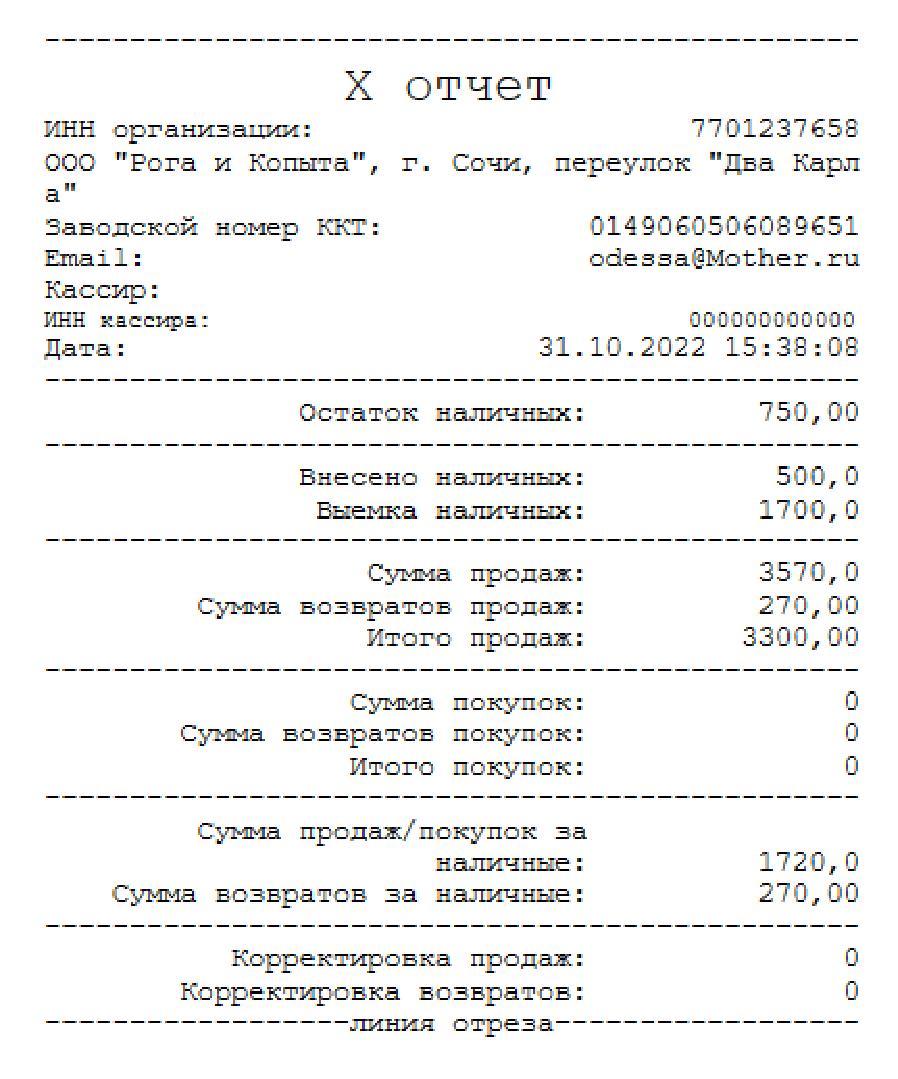
\includegraphics[width=0.5\linewidth]{xotchet} 
	\caption{Формат X-отчёта}
	\label{xotchet:image}
\end{figure}

\section{Техническое задание}


\subsection{Основание для разработки}
Основанием для разработки является задание на выпускную квалификационную работу бакалавра "<Программно-информационная система оптимизации ресторанного бизнеса">.

\subsection{Цель и назначение разработки}
Основной задачей выпускной квалификационной работы является разработка программы для оптимизации ресторанного бизнеса. Для достижения поставленной цели необходимо решить следующие задачи: 
\begin{itemize}
	\item провести анализ предметной области; 
	\item разработать концептуальную модель программы; 
	\item спроектировать базу данных;
	\item разработать механизм формирования финансовых отчётов;
	\item реализовать процесс создания технологических карт;
	\item интегрировать данные сотрудников в систему.
\end{itemize}

\subsection{Требования пользователя к интерфейсу программы}
Программа должна включать в себя:
\begin{itemize}
    \item авторизацию;
    \item доступы для управляющего, администратора, повара, официант;
    \item окно ввода заказа;
    \item модуль для управления данными сотрудников;
    \item возможность создания технологических карт;
    \item формирование финансовых отчётов.
\end{itemize}

Композиция шаблона окна авторизации представлена на рисунке ~\ref{compositionin:image} и состоит из:
\begin{itemize}
	\item поле для ввода кода (1);
	\item экранная клавиатура (2);
	\item кнопка для очистки поля (3);
	\item кнопка для подтверждения ввода пароля (4).
\end{itemize}
\begin{figure}[ht]
	\centering
	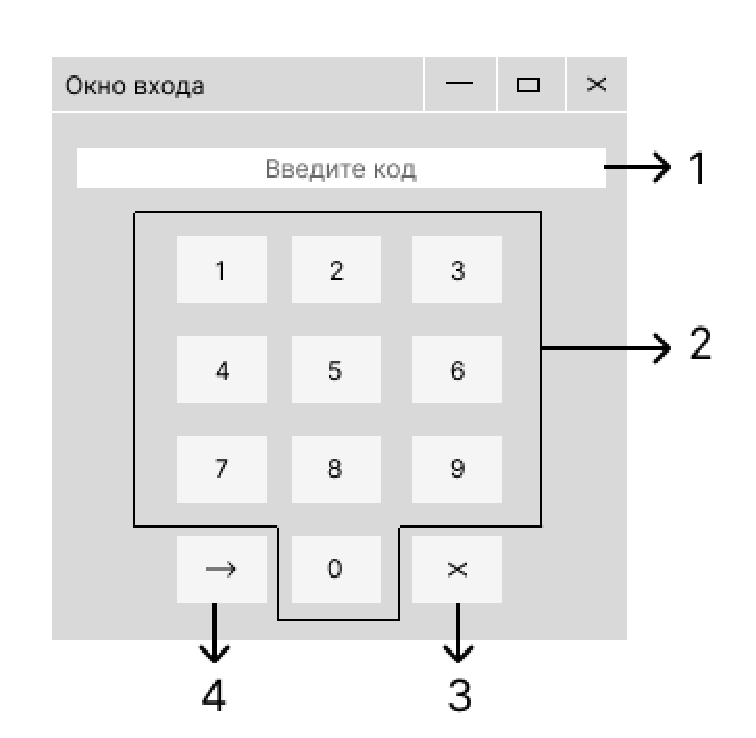
\includegraphics[width=0.5\linewidth]{compositionin}
	\caption{Композиция шаблона окна авторизации}
	\label{compositionin:image}
\end{figure}

Схема окна ввода заказа продемонстрирована на рисунке ~\ref{compositionzakaz:image} и содержит следующие компоненты:
\begin{itemize}
	\item поле для вывода номера заказа и стола (1);
	\item таблицы вывода данных о блюдах (2);
	\item кнопка для добавления скидки (3);
	\item поле для подсчёта итоговой стоимости (4);
	\item кнопка для печати заказа (5);
	\item кнопка для оплаты заказа(6);
	\item кнопки с названием блюда для добавления их в заказ (7);
	\item кнопки с названием категорий для выбора блюд (8).
\end{itemize}
\begin{figure}[ht]
	\centering
	\includegraphics[width=0.8\linewidth]{compositionzakaz}
	\caption{Композиция шаблона окна заказа}
	\label{compositionzakaz:image}
\end{figure} 

\newpage
Шаблон модуля для работы с базой данных (управление данными сотрудников, редактирование меню) изображен на рисунке ~\ref{composition1:image}. Он включает в себя:
\begin{itemize}
	\item кнопка для добавления данных (1);
	\item кнопка для редактирования данных (2);
	\item кнопка для удаления данных (3);
	\item кнопка для поиска данных (4);
	\item кнопка для поиска в таблице (5);
	\item таблица для просмотра данных из БД (6).
\end{itemize}
\begin{figure}[ht]
	\centering
	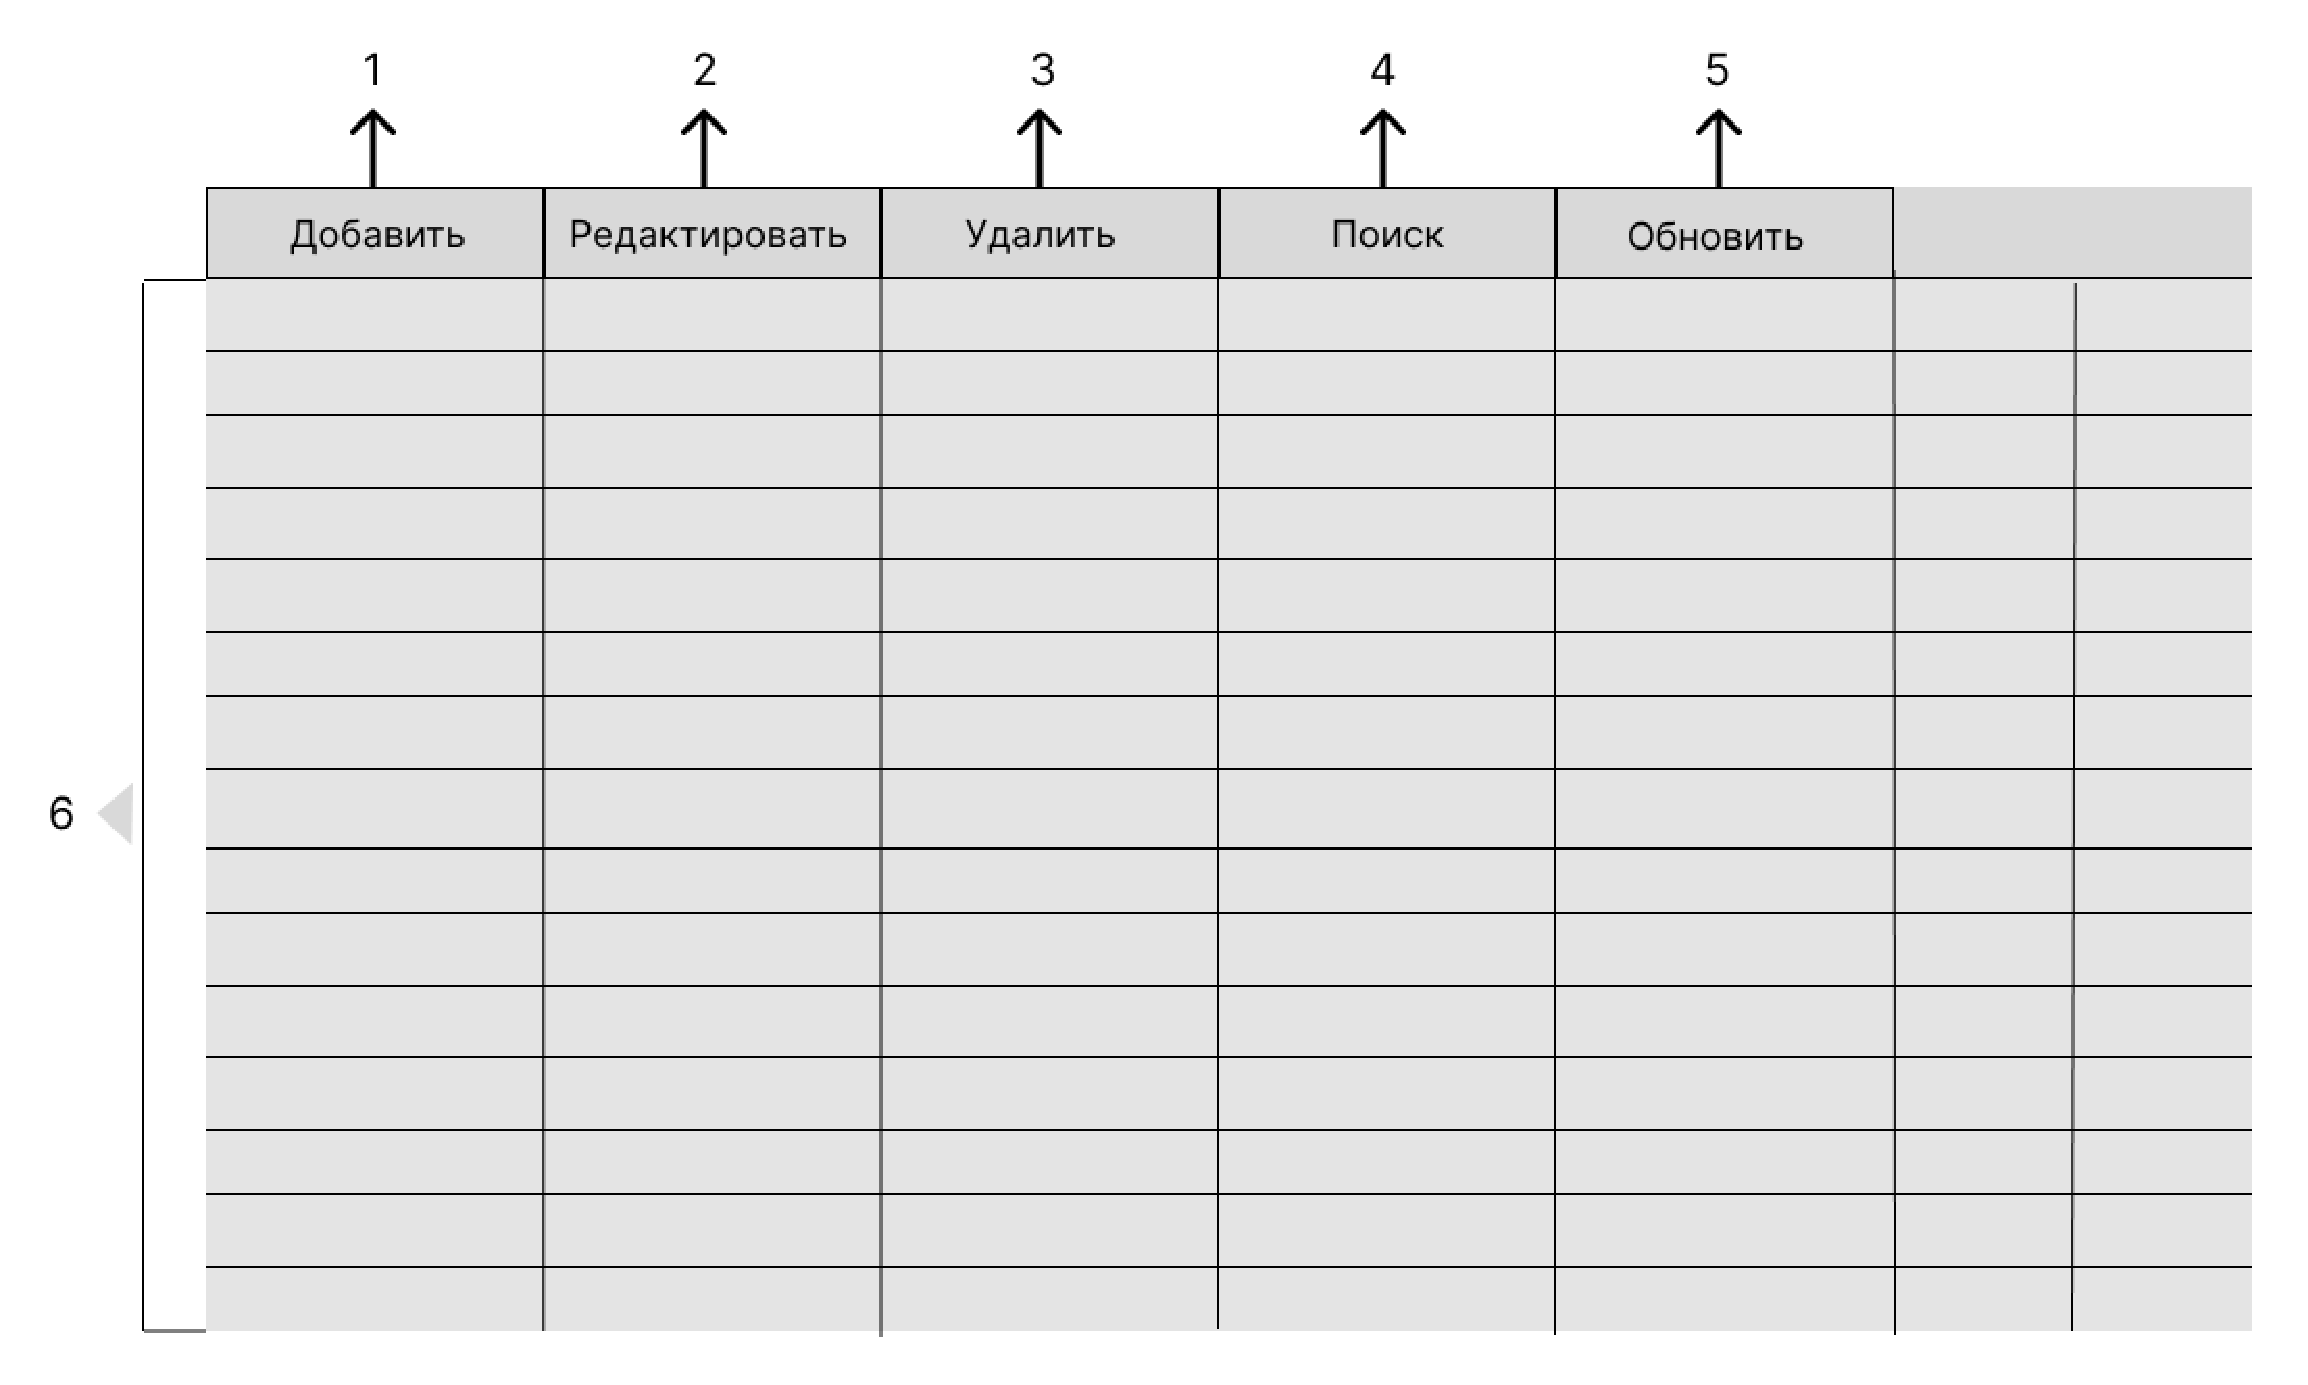
\includegraphics[width=0.7\linewidth]{composition1}
	\caption{Композиция шаблона модуля работы с базой данных}
	\label{composition1:image}
\end{figure}

\newpage
Макет окна для создания технологических карт проиллюстрирован на рисунке ~\ref{compositiontex:image} и состоит из:
\begin{itemize}
	\item поле для ввода названия блюда (1);
	\item поле для ввода описания блюда (2);
	\item поле для ввода рецепта (3);
	\item кнопка для редактирования данных ингредиентов в таблице (4);
	\item кнопка для добавления ингредиентов в таблицу (5);
	\item таблица для добавления данных об ингредиентах (6);
	\item поле для ввода количества белков (7);
	\item поле для ввода количества жиров (8);
	\item поле для ввода количества углеводов (9);
	\item поле для ввода количества калорий (10);
	\item кнопка для сохранения данных в БД (11);
	\item кнопка для удаления данных из таблицы ингредиентов (12);
\end{itemize}
\begin{figure}[ht]
	\centering
	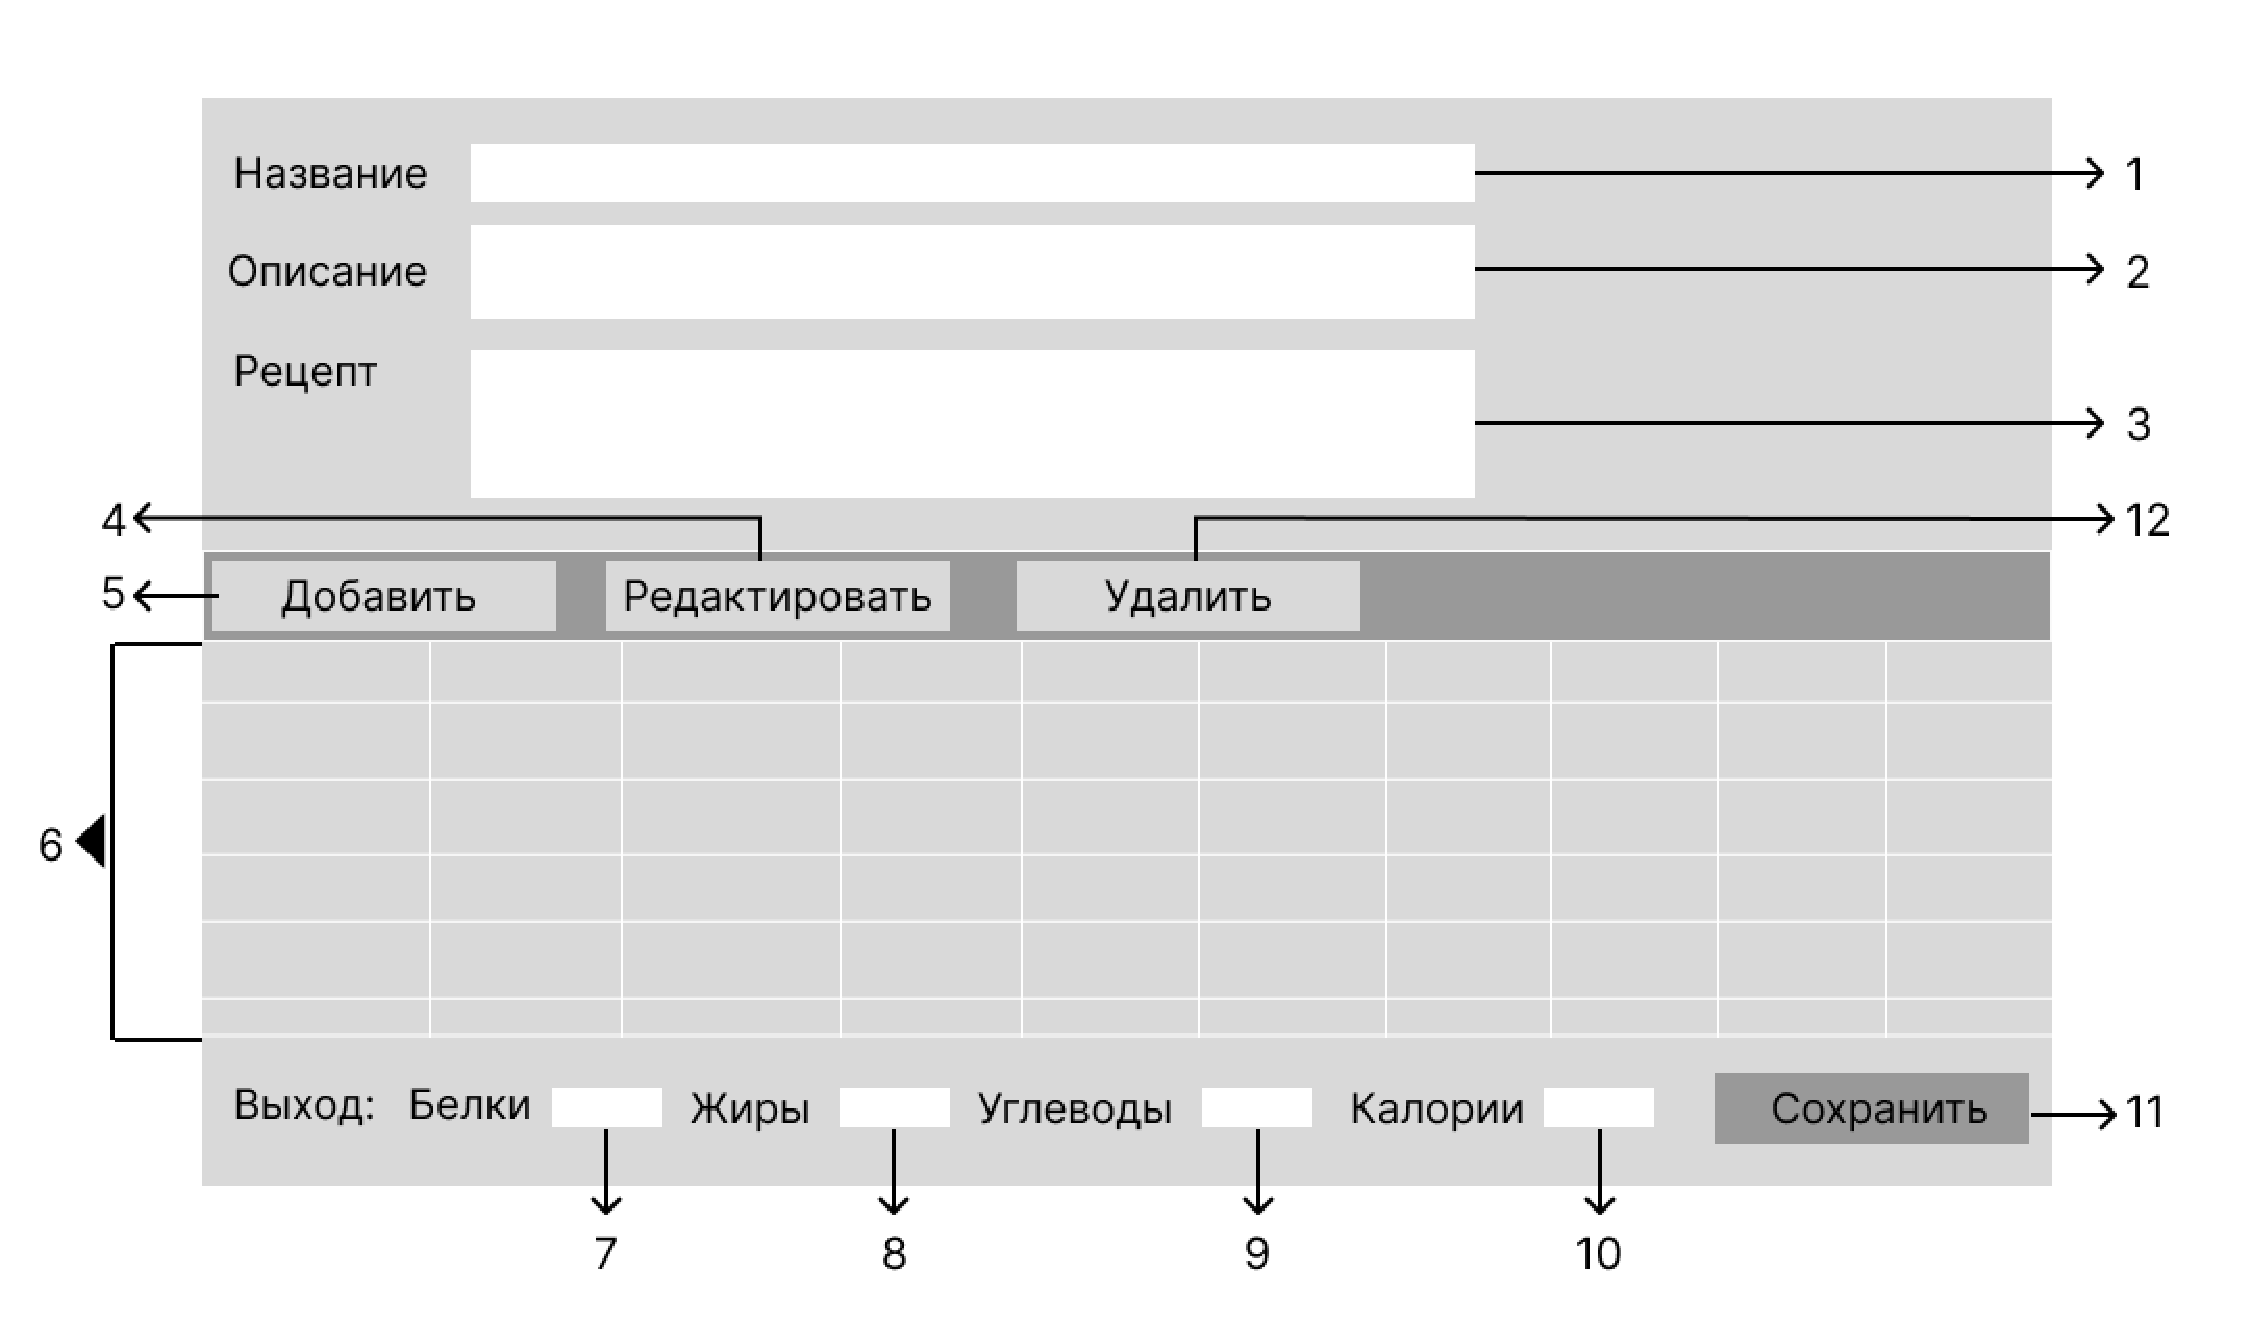
\includegraphics[width=0.8\linewidth]{compositiontex}
	\caption{Композиция шаблона модуля для создания технологических карт}
	\label{compositiontex:image}
\end{figure}


\newpage
\subsection{Моделирование вариантов использования}

Для разрабатываемой системы была реализована модель, обеспечивающая наглядное представление вариантов использования программы с помощью унифицированного языка визуального моделирования UML. 

В диаграмме вариантов (прецедентов) проектируемая система рассматривается как ряд прецедентов, предоставляемых системой актерами - пользователями или другими компьютерными системами, взаимодействующими с данной. Варианты использования системы изображаются в виде овалов, внутри которых пишется название сценария \cite{uml}. Сценарий взаимодействия позволяет пользователям достигать целей использования программы с помощью функциональной системы. Связь между актёрами и вариантами использования реализуют с помощью ассоциаций. 

Использование UML для визуального представления работы системы позволяет выявить ключевые взаимодействия и зависимости между элементами программы, что упрощает понимание требований и возможностей системы, а также способствует более эффективной разработке и тестированию. 

На основании анализа предметной области в программе должны быть реализованы следующие прецеденты:
\begin{enumerate}
\item Добавление, просмотр и редактирование данных о сотруднике.
\item Создание, просмотр и редактирование заказа.
\item Создание, просмотр и редактирование технологических карт.
\item Обработка платежа.
\item Создание и просмотр финансовых отчётов.
\end{enumerate}

Программа имеет четыре группы пользователей с разными правами: управляющий, старший повар, администратор и официант. 
\newline
Управляющему должны быть доступны следующие функции:
\begin{enumerate}
	\item Добавление, просмотр и редактирование данных о сотрудниках.
	\item Создание, просмотр и редактирование данных о должностях.
	\item Редактирование данных заведения.
	\item Управление количеством столов.
	\item Редактирование типов оплаты.
	\item Назначение размеров скидки.
\end{enumerate}
На рисунке ~\ref{diagramyprav:image} изображены прецеденты для управляющего.
\begin{figure}[ht]
	\centering
	\includegraphics[width=1\linewidth]{diagramyprav}
	\caption{Диаграмма прецедентов для категории пользователей - управляющий}
	\label{diagramyprav:image}
\end{figure}
\newline
Старшему повару должны быть доступны следующие функции:
\begin{enumerate}
	\item Добавление, просмотр и редактирование данных о блюдах.
	\item Создание, просмотр и редактирование технологических карт.
	\item Добавление категорий меню.
	\item Добавление ингредиентов.
\end{enumerate}
На рисунке ~\ref{diagramlshef:image} изображены прецеденты для старшего повара.
\begin{figure}[ht]
	\centering
	\includegraphics[width=1\linewidth]{diagramlshef}
	\caption{Диаграмма прецедентов для категории пользователей - старший повар}
	\label{diagramlshef:image}
\end{figure}
\newpage
Официанту должны быть доступны следующие функции:
\begin{enumerate}
	\item Создание, редактирование, удаление заказа.
	\item Передача заказа на кухню.
	\item Формирование счёта.
	\item Обработка оплаты.
	
\end{enumerate}
На рисунке ~\ref{diagramoff:image} изображены прецеденты для официанта ресторана.
\begin{figure}[ht]
	\centering
	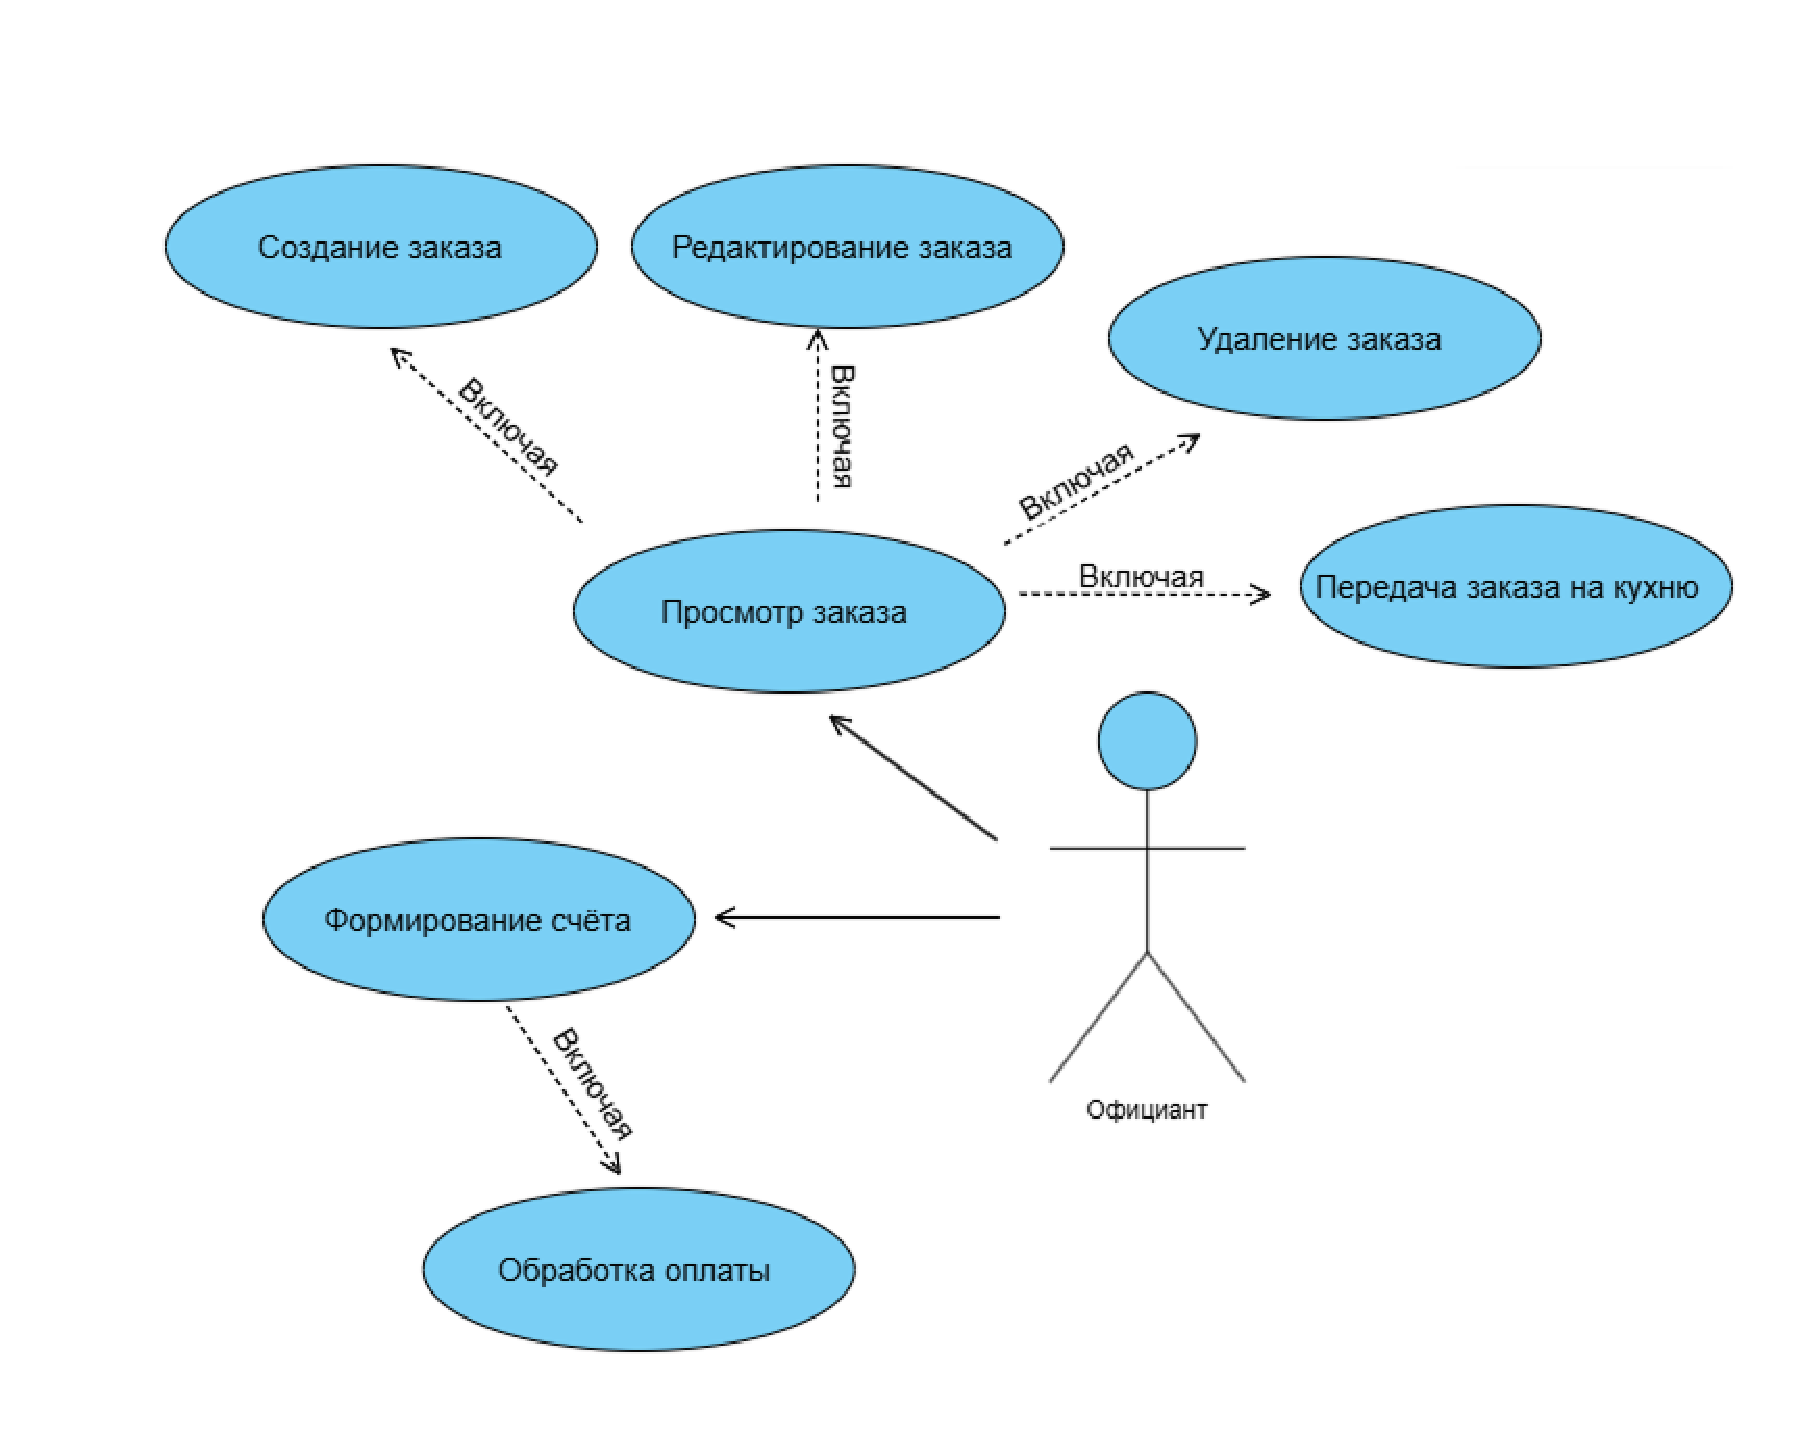
\includegraphics[width=1\linewidth]{diagramoff}
	\caption{Диаграмма прецедентов для категории пользователей - официант}
	\label{diagramoff:image}
\end{figure}
\newpage
Администратору должны быть доступны следующие функции:
\begin{enumerate}
	\item Просмотр отчёта о закрытии смены.
	\item Просмотр отчёта о движении денежных средств.
	\item Просмотр данных закрытых заказов.
\end{enumerate}
На рисунке ~\ref{diagramadmin:image} изображены прецеденты для администратора ресторана.
\begin{figure}[ht]
	\centering
	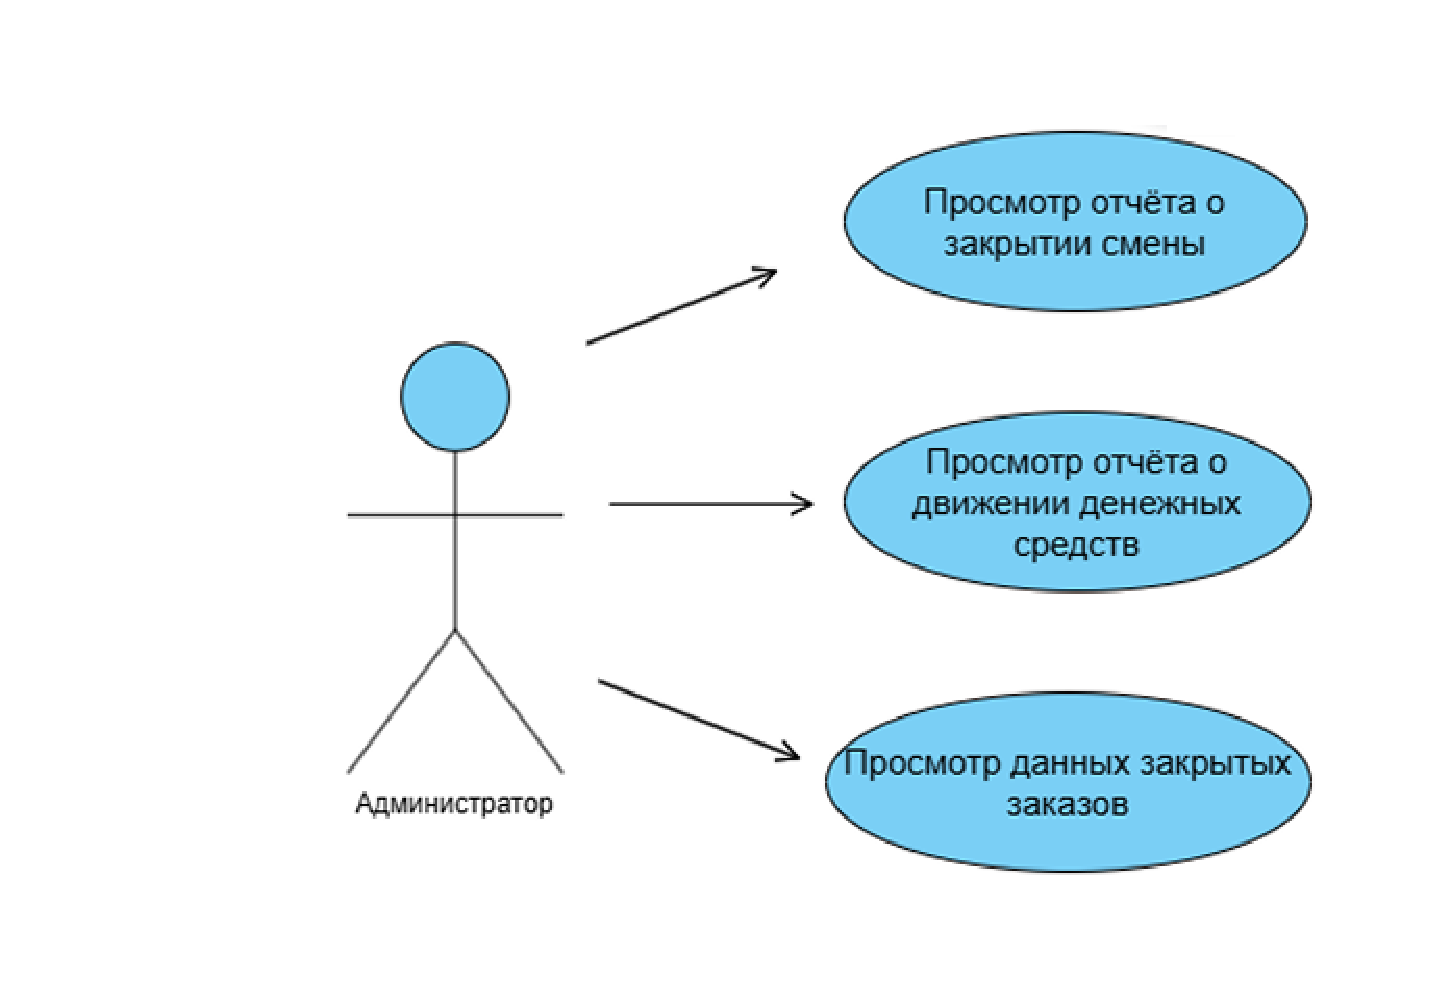
\includegraphics[width=0.7\linewidth]{diagramadmin}
	\caption{Диаграмма прецедентов для категории пользователей - администратор}
	\label{diagramadmin:image}
\end{figure}


\newpage
\subsection{Требования к оформлению документации}

Разработка программной документации и программного изделия должна производиться согласно ГОСТ 19.102-77 и ГОСТ 34.601-90. Единая система программной документации.

\section{Технический проект}


\subsection{Общая характеристика организации решения задачи}
Необходимо спроектировать и разработать программно-информационную систему, которая способствует оптимизации ресторанного бизнеса.  
Программа представляет собой набор модулей, которые помогут оптимизировать и автоматизировать такие процессы, как управление заказами и персоналом, учет ресурсов, формирование отчетности.
Программа написана на языке программирования Python.


\subsection{Обоснование выбора технологии проектирования}
На сегодняшний день информационный рынок, поставляющий программные решения в выбранной сфере, предлагает множество продуктов, позволяющих достигнуть поставленной цели – разработки приложения.


\subsubsection{Описание используемых технологий и языков программирования}
В процессе разработки программного продукта был использован язык программирования Python, его объекты и библиотеки, а также объектно-реляционная система управления базами данных PostgreSQL.


\subsubsection{Язык программирования Python}
Python — высокоуровневый язык программирования. Он широко используется во всем мире для самых разных целей — базы данных и обработка текстов, встраивание интерпретатора в игры, программирование GUI и быстрое создание прототипов (RAD)\cite{python}.

\paragraph{Библиотека Tkiner}
Tkinter — это модуль Python, который работает с библиотекой Tk - стандартной библиотекой Python \cite{tkiner}. С помощью данной библиотеки было реализовано множество проектов, благодаря ее доступности, универсальности и эффективности. Библиотека представляет собой набор виджетов, например, кнопки, метки, текстовые поля. Не менее важным является тот факт, что tkiner поддерживает кроссплатформенность, что позволяет, приложениям работать на различных операционных системах.

\subsubsection{PostgerSQL} 


PostgreSQL, или просто postgres, –  мощная объектно-реляционная СУБД с открытым исходным кодом, которая позволяет создавать высоконагруженные базы данных большого объема \cite{postgrestermin}. Преимуществами данной системы является её расширяемость, техническое совершенство и совместимость. Используют postgreSQL в различных сферах, начиная от коммерческих продуктов и заканчивая госучреждениями. Плюсом posgres является её кросс-платформленность, что позволяет использовать готовый продукт в большинстве современных операционных систем.


\paragraph{Достоинства PostgerSQL}
С точки зрения пользователя PosqreSQL обладает следующими преимуществами:
\begin{itemize}
 	\item регулярный обновления;
 	\item общирная документация;
 	\item широкий арсенал расширений;
 	\item бесплатный исходный код;
 	\item возможность автоматизированного решения администраторских задач;
 	\item интеграция с другими СУБД \cite{postgres}.
\end{itemize}
PosgreSQL также будет хорошим выбором и с точки зрения бизнеса:
\begin{itemize}
	\item бесплатная лицензия;
	\item система хорошо масштабируется;
	\item posqres обеспечивает высокую производительность;
	\item не имеет ограничений на количество развернутых экземпляров;
	\item является кросс-платформленным ПО;
	\item обладает высокой надежностью.
\end{itemize}	
	


\subsection{Диаграмма компонентов и схема обмена данными между файлами компонента}

Диаграмма компонентов — это, фактически, список артефактов, из которых состоит моделируемая система, с указанием некоторых отношений между артефактами \cite{components}.
В данной диаграмме компонентом считается как программные составляющие, например, база данных и пользовательский интерфейс, так и аппаратные - схема, устройство. На рисунке  ~\ref{componetdiag:image} представлена диаграмма компонентов для проектируемой системы. На данной диаграмме изображён сервер, база данных, кассовый терминал и модули системы.
\begin{figure}[ht]
\centering
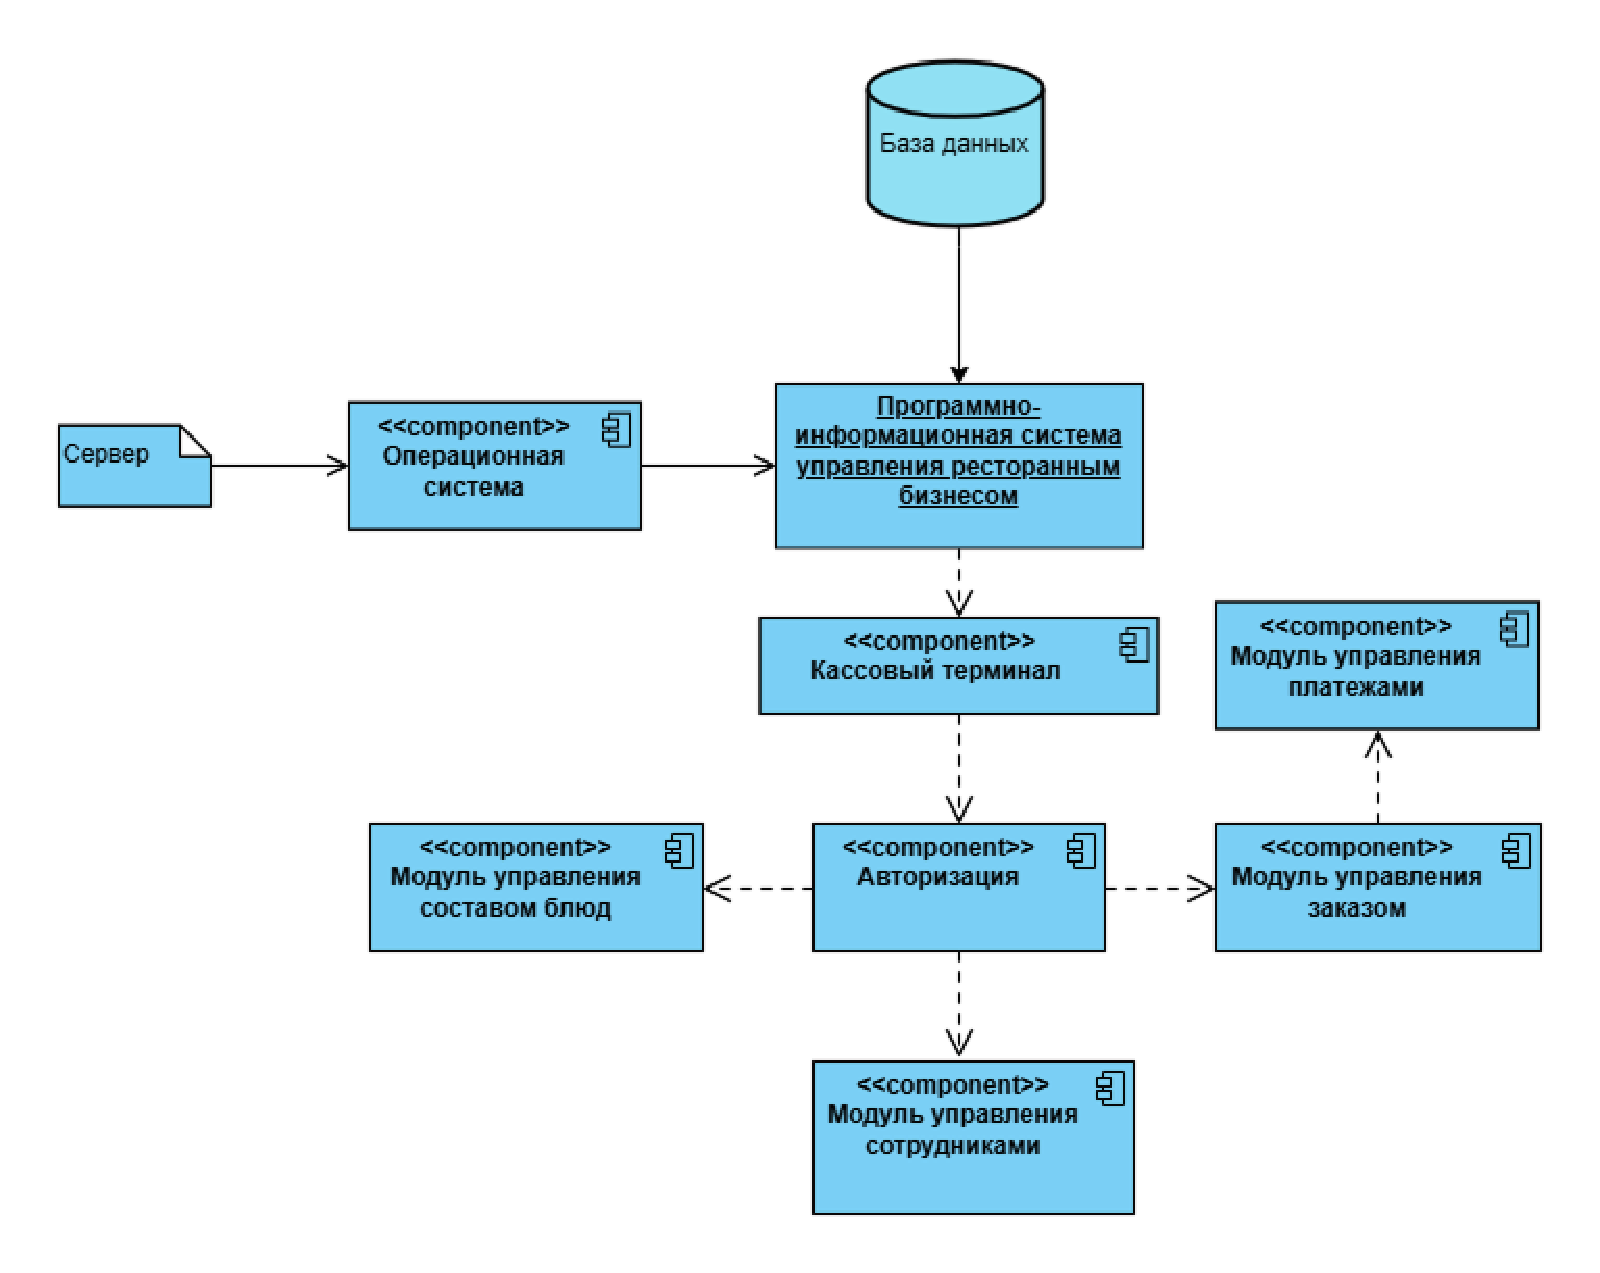
\includegraphics[width=1\linewidth]{componetdiag}
\caption{Диаграмма компонентов}
\label{componetdiag:image}
\end{figure}


\subsection{Структура базы данных}
Сущности и отношение между таблицами базы данных отражены на рисунке~\ref{erd:image}.
\begin{figure}[ht]
	\centering
	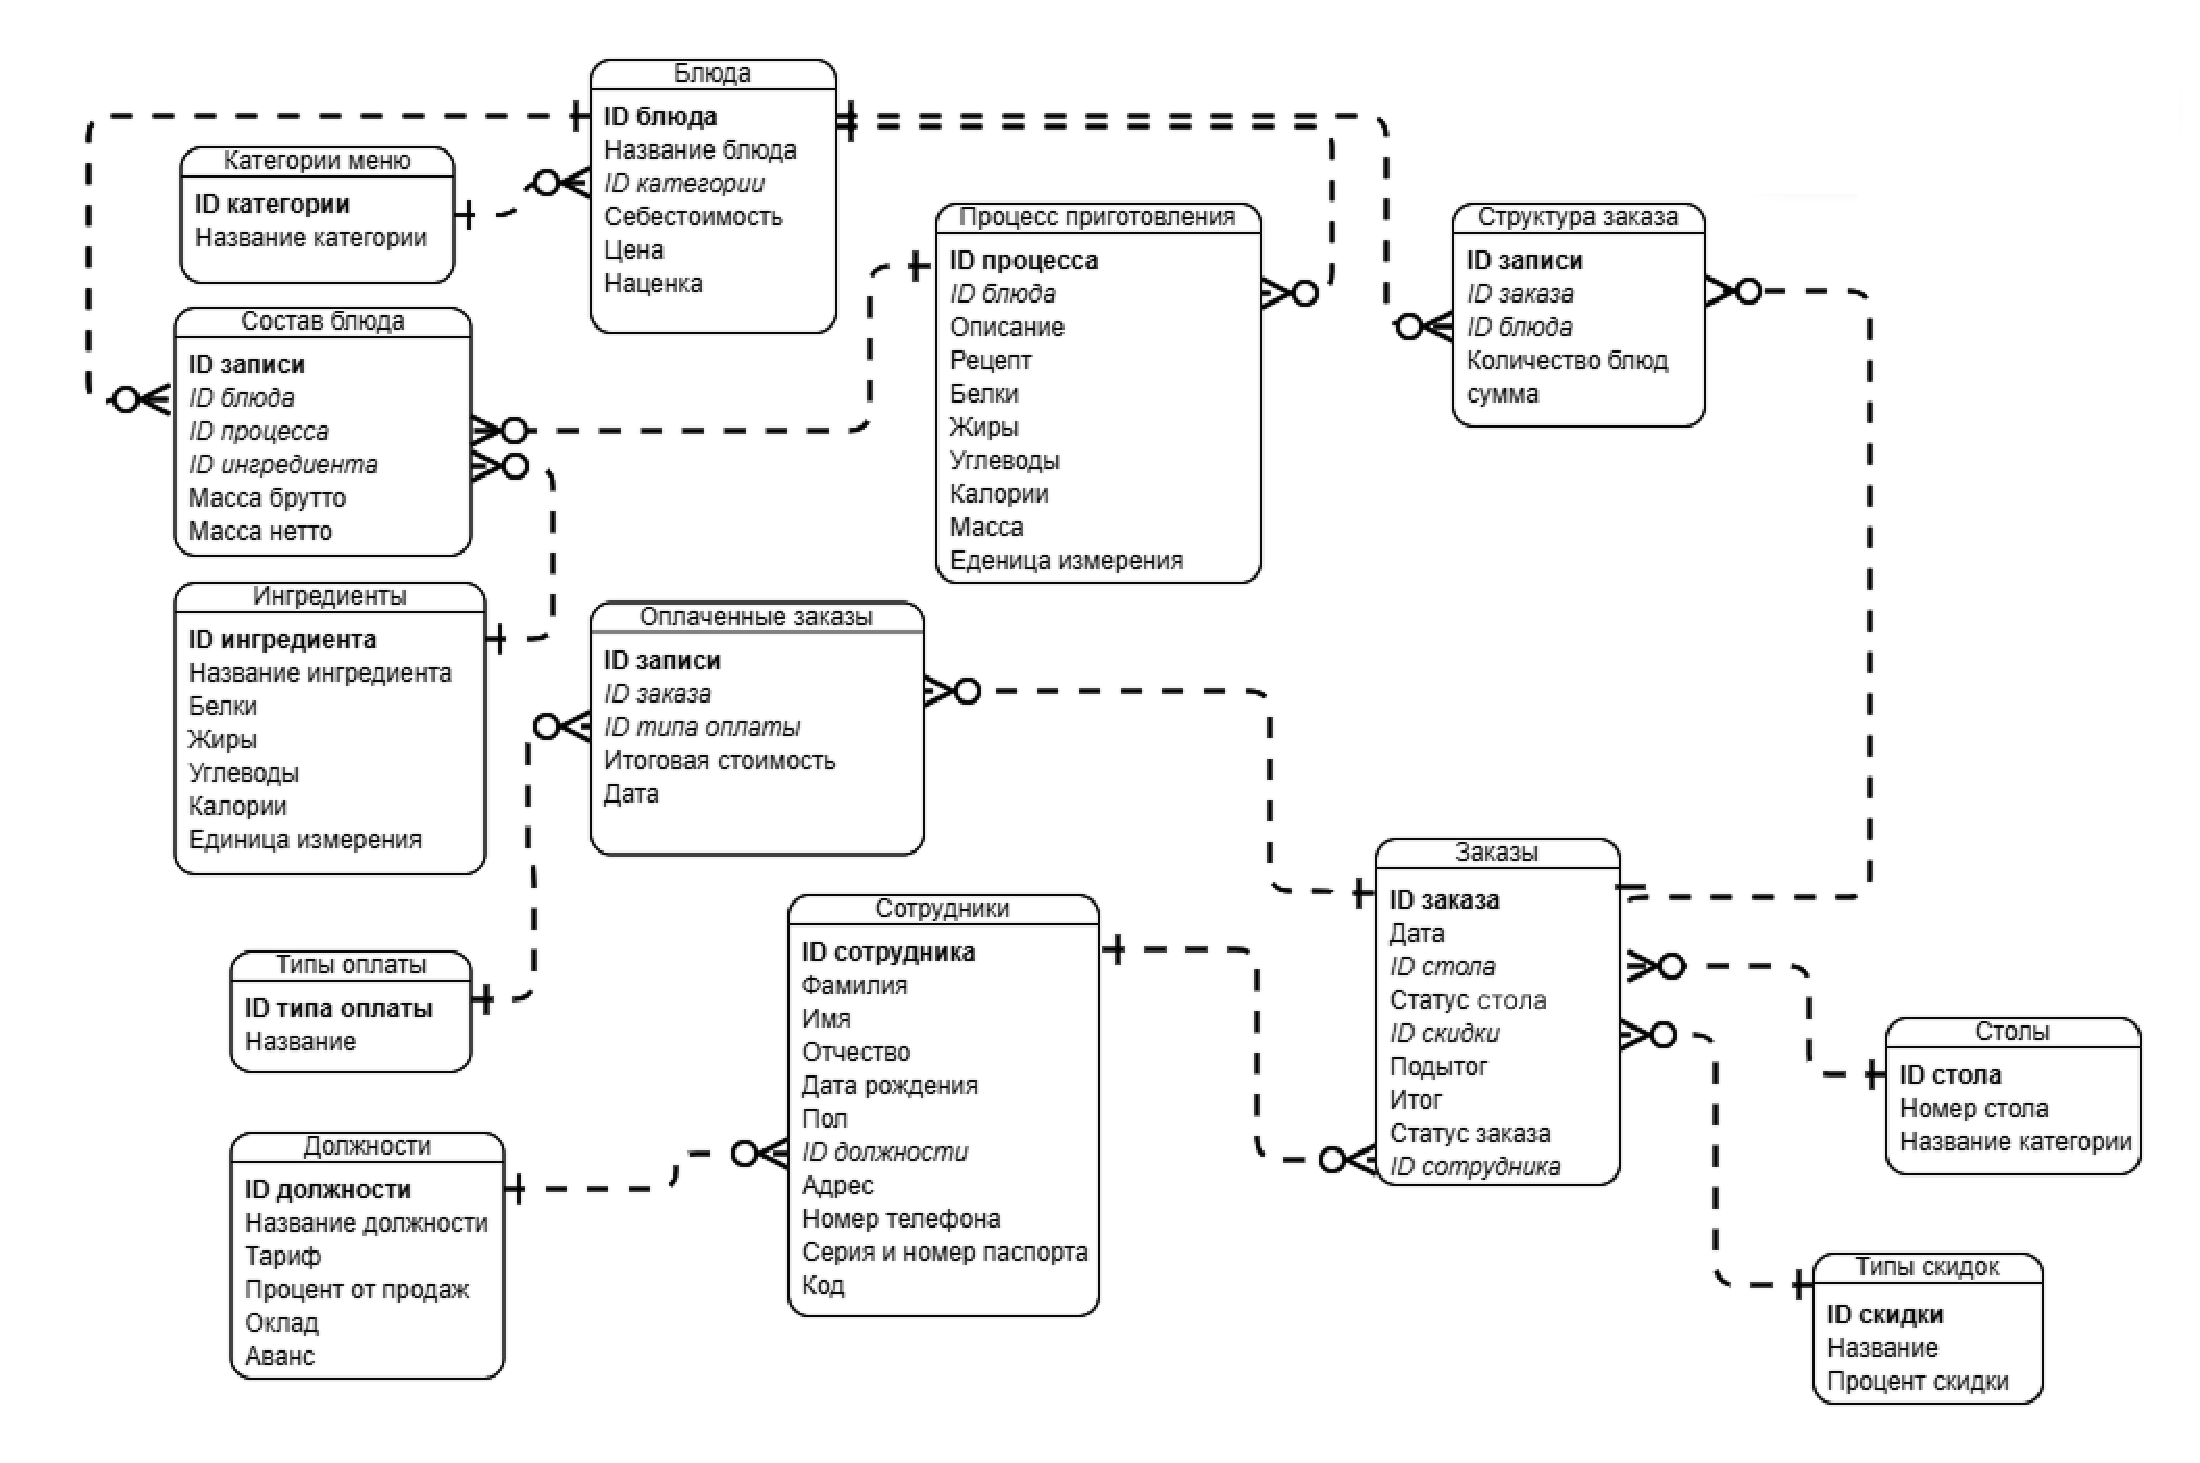
\includegraphics[width=1\linewidth]{erd}
	\caption{ER-диаграмма}
	\label{erd:image}
\end{figure}
\newline
В таблице \ref{staff:table} представлена структура таблицы staff.
\begin{xltabular}{\textwidth}{|l|p{4.5cm}|p{2.2cm}|X|}
	\caption{Таблица staff\label{staff:table}}\\ \hline
	\centrow  Тип ключа & \centrow Имя столбца & \centrow  Тип данных & \centrow Обязательность \\ \hline
	\endfirsthead
	\continuecaption{Продолжение таблицы \ref{staff:table}} 
	\centrow  Тип ключа & \centrow Имя столбца & \centrow  Тип данных & \centrow Обязательность   \\ \hline
	\finishhead
	primary key & id\_staff & Integer & true  \\ \hline 
	~ & last\_name & Text & true  \\ \hline 
	~ & first\_name & Text & true  \\ \hline 
	~ & middle\_name & Text & false \\ \hline
	~ & birth & Date & true  \\ \hline 
	~ & gender & Text & true  \\ \hline 
	foreing key & id\_post & Integer & true \\ \hline 
	~ & adress & Text & false\\ \hline 
	~ & phone\_number & Bigint & true  \\ \hline
	~ & ser\_num\_pass & Bigint & false \\ \hline
	~ & code & Integer & true
\end{xltabular}


В таблице \ref{post:table} представлена структура таблицы post.
\begin{xltabular}{\textwidth}{|l|p{4.5cm}|p{2.2cm}|X|}
	\caption{Таблица post\label{post:table}}\\ \hline
	\centrow  Тип ключа & \centrow Имя столбца & \centrow  Тип данных & \centrow Обязательность \\ \hline
	\endfirsthead
	\continuecaption{Продолжение таблицы \ref{post:table}} 
	\centrow  Тип ключа & \centrow Имя столбца & \centrow  Тип данных & \centrow Обязательность   \\ \hline
	\finishhead
	primary key & id\_post & Integer & true \\ \hline 
	~ & name\_post & Text & true  \\ \hline 
	~ & rate & Numeric & true  \\ \hline 
	~ & percent & Text & false  \\ \hline
	~ & selary & Date & false\\ \hline 
	~ & advance & Text & false    
\end{xltabular}

В таблице \ref{order:table} представлена структура таблицы order.
\begin{xltabular}{\textwidth}{|l|p{4.5cm}|p{2.2cm}|X|}
	\caption{Таблица order\label{order:table}}\\ \hline
	\centrow  Тип ключа & \centrow Имя столбца & \centrow  Тип данных & \centrow Обязательность \\ \hline
	\endfirsthead
	\continuecaption{Продолжение таблицы \ref{order:table}} 
	\centrow  Тип ключа & \centrow Имя столбца & \centrow  Тип данных & \centrow Обязательность   \\ \hline
	\finishhead
	primary key & id\_order & Integer & true \\ \hline 
	~ & date & Date & true \\ \hline 
	foreing key & id\_table & Text & true \\ \hline 
	~ & status\_ordere & Integer & true  \\ \hline
	foreing key & id\_sale & Text & true  \\ \hline 
	~ & summary & Numeric & true \\ \hline 
	~ & result & Integer & true \\ \hline 
	~ & order\_condition & Text & false
\end{xltabular}

В таблице \ref{tables:table} представлена структура таблицы tables.
\begin{xltabular}{\textwidth}{|l|p{4.5cm}|p{2.2cm}|X|}
	\caption{Таблица tables\label{tables:table}}\\ \hline
	\centrow  Тип ключа & \centrow Имя столбца & \centrow  Тип данных & \centrow Обязательность \\ \hline
	\endfirsthead
	\continuecaption{Продолжение таблицы \ref{tables:table}} 
	\centrow  Тип ключа & \centrow Имя столбца & \centrow  Тип данных & \centrow Обязательность   \\ \hline
	\finishhead
	primary key & id\_tabel & Integer & true \\ \hline 
	~ & number\_tabel & Integer & true \\ \hline 
	~ & name\_tabel & Text & true 
\end{xltabular}

В таблице \ref{paytype:table} представлена структура таблицы pay\_types.
\begin{xltabular}{\textwidth}{|l|p{4.5cm}|p{2.2cm}|X|}
	\caption{Таблица pay\_types\label{paytype:table}}\\ \hline
	\centrow  Тип ключа & \centrow Имя столбца & \centrow  Тип данных & \centrow Обязательность \\ \hline
	\endfirsthead
	\continuecaption{Продолжение таблицы \ref{paytype:table}} 
	\centrow  Тип ключа & \centrow Имя столбца & \centrow  Тип данных & \centrow Обязательность   \\ \hline
	\finishhead
	primary key & id\_type & Integer & true \\ \hline 
	~ & name\_type & Text & true 
\end{xltabular}

В таблице \ref{structureorder:table} представлена структура таблицы structure\_order.
\begin{xltabular}{\textwidth}{|l|p{4.5cm}|p{2.2cm}|X|}
	\caption{Таблица structure\_order\label{structureorder:table}}\\ \hline
	\centrow  Тип ключа & \centrow Имя столбца & \centrow  Тип данных & \centrow Обязательность \\ \hline
	\endfirsthead
	\continuecaption{Продолжение таблицы \ref{structureorder:table}} 
	\centrow  Тип ключа & \centrow Имя столбца & \centrow  Тип данных & \centrow Обязательность   \\ \hline
	\finishhead
	primary key & id\_record & Integer & true \\ \hline 
	foreing key & id\_order & Integer & true \\ \hline 
	foreing key & id\_dish & Integer & true \\ \hline 
	~ & status\_ordere & Integer & true  \\ \hline 
	~ & dish\_quantity & Integer & true \\ \hline 
	~ & sum & Numeric & true  
\end{xltabular}

В таблице \ref{paidorders:table} представлена структура таблицы paid\_orders.
\begin{xltabular}{\textwidth}{|l|p{4.5cm}|p{2.2cm}|X|}
	\caption{Таблица paid\_orders\label{paidorders:table}}\\ \hline
	\centrow  Тип ключа & \centrow Имя столбца & \centrow  Тип данных & \centrow Обязательность \\ \hline
	\endfirsthead
	\continuecaption{Продолжение таблицы \ref{paidorders:table}} 
	\centrow  Тип ключа & \centrow Имя столбца & \centrow  Тип данных & \centrow Обязательность   \\ \hline
	\finishhead
	primary key & id\_data & Integer & true \\ \hline 
	foreing key & id\_order & Integer & true \\ \hline 
	foreing key & id\_pay\_type & Text & true \\ \hline 
	~ & sum & Integer & true  \\ \hline
	~ & date & Text & true  \\ \hline 
	~ & summary & Numeric & true \\ \hline 
	~ & result & Integer & true \\ \hline 
	~ & order\_condition & Text & true
\end{xltabular}

В таблице \ref{paytypes:table} представлена структура таблицы pay\_types.
\begin{xltabular}{\textwidth}{|l|p{4.5cm}|p{2.2cm}|X|}
	\caption{Таблица pay\_types\label{paytypes:table}}\\ \hline
	\centrow  Тип ключа & \centrow Имя столбца & \centrow  Тип данных & \centrow Обязательность \\ \hline
	\endfirsthead
	\continuecaption{Продолжение таблицы \ref{paytypes:table}} 
	\centrow  Тип ключа & \centrow Имя столбца & \centrow  Тип данных & \centrow Обязательность   \\ \hline
	\finishhead
	primary key & id\_type & Integer & true \\ \hline 
	~ & name\_type & Text & true
\end{xltabular}

В таблице \ref{menudishprocess:table} представлена структура таблицы menu\_dish\_process.
\begin{xltabular}{\textwidth}{|l|p{4.5cm}|p{2.2cm}|X|}
	\caption{Таблица menu\_dish\_process\label{menudishprocess:table}}\\ \hline
	\centrow  Тип ключа & \centrow Имя столбца & \centrow  Тип данных & \centrow Обязательность \\ \hline
	\endfirsthead
	\continuecaption{Продолжение таблицы \ref{menudishprocess:table}} 
	\centrow  Тип ключа & \centrow Имя столбца & \centrow  Тип данных & \centrow Обязательность   \\ \hline
	\finishhead
	primary key & id\_process & Integer & true  \\ \hline 
	foreing key & id\_dish & Integer & true  \\ \hline 
	~ & description & Text & true  \\ \hline 
	~ & recept & Text & false \\ \hline
	~ & birth & Date & false  \\ \hline 
	~ & proteins & Numeric & false  \\ \hline 
	~ & fats & Numeric & false \\ \hline 
	~ & carbohydrates & Numeric & false\\ \hline 
	~ & calories & Numeric & false  \\ \hline
	~ & massa & Numeric & false \\ \hline
	~ & ed\_ismereni & Text & false
\end{xltabular}

В таблице \ref{dish:table} представлена структура таблицы menu\_dishes.
\begin{xltabular}{\textwidth}{|l|p{4.5cm}|p{2.2cm}|X|}
	\caption{Таблица menu\_dishes\label{dish:table}}\\ \hline
	\centrow  Тип ключа & \centrow Имя столбца & \centrow  Тип данных & \centrow Обязательность \\ \hline
	\endfirsthead
	\continuecaption{Продолжение таблицы \ref{dish:table}} 
	\centrow  Тип ключа & \centrow Имя столбца & \centrow  Тип данных & \centrow Обязательность   \\ \hline
	\finishhead
	primary key & id\_dish & Integer & true \\ \hline 
	~ & name\_dish & Text & true  \\ \hline
	foreing key  & id\_category & Integer & true  \\ \hline 
	~ & cost\_dish & Numeric & true \\ \hline
	~ & price\_dish & Numeric & true  \\ \hline 
	~ & extra\_dish & Numeric & true 
\end{xltabular}

В таблице \ref{category:table} представлена структура таблицы menu\_category.
\begin{xltabular}{\textwidth}{|l|p{4.5cm}|p{2.2cm}|X|}
	\caption{Таблица pay\_types\label{category:table}}\\ \hline
	\centrow  Тип ключа & \centrow Имя столбца & \centrow  Тип данных & \centrow Обязательность \\ \hline
	\endfirsthead
	\continuecaption{Продолжение таблицы \ref{category:table}} 
	\centrow  Тип ключа & \centrow Имя столбца & \centrow  Тип данных & \centrow Обязательность   \\ \hline
	\finishhead
	primary key & id\_category & Integer & true \\ \hline 
	~ & name\_category & Text & true
\end{xltabular}

В таблице \ref{composition:table} представлена структура таблицы menu\_dish\_composition.
\begin{xltabular}{\textwidth}{|l|p{4.5cm}|p{2.2cm}|X|}
	\caption{Таблица menu\_dish\_composition\label{composition:table}}\\ \hline
	\centrow  Тип ключа & \centrow Имя столбца & \centrow  Тип данных & \centrow Обязательность \\ \hline
	\endfirsthead
	\continuecaption{Продолжение таблицы \ref{composition:table}} 
	\centrow  Тип ключа & \centrow Имя столбца & \centrow  Тип данных & \centrow Обязательность   \\ \hline
	\finishhead
	primary key & id\_composition & Integer & true  \\ \hline 
	foreing key & id\_dish & Integer & true  \\ \hline 
	foreing key & id\_process & Integer & true  \\ \hline 
	foreing key & id\_ingredient & Integer & true  \\ \hline 
	~ & massa\_brytto & Numeric & true  \\ \hline 
	~ & massa\_netto & Numeric & true 
\end{xltabular}

В таблице \ref{ingredients:table} представлена структура таблицы menu\_ingredient.
\begin{xltabular}{\textwidth}{|l|p{4.5cm}|p{2.2cm}|X|}
	\caption{Таблица menu\_ingredient\label{ingredients:table}}\\ \hline
	\centrow  Тип ключа & \centrow Имя столбца & \centrow  Тип данных & \centrow Обязательность \\ \hline
	\endfirsthead
	\continuecaption{Продолжение таблицы \ref{ingredients:table}} 
	\centrow  Тип ключа & \centrow Имя столбца & \centrow  Тип данных & \centrow Обязательность   \\ \hline
	\finishhead
	primary key & id\_ingredient & Integer & true  \\ \hline 
	~ & name\_ingredient & Text & true  \\ \hline
	~ & proteins & Numeric & false  \\ \hline 
	~ & fats & Numeric & false \\ \hline 
	~ & carbohydrates & Numeric & false\\ \hline 
	~ & calories & Numeric & false  \\ \hline
	~ & massa & Numeric & false \\ \hline
	~ & ed\_ismereni & Text & false
\end{xltabular}



\ifПрактика{}\else{
   \input{РабочийПроект}
   \input{Заключение}
}\fi
\addcontentsline{toc}{section}{СПИСОК ИСПОЛЬЗОВАННЫХ ИСТОЧНИКОВ}

\begin{thebibliography}{9}

    \bibitem{tkiner} Букунов С. В. Разработка приложений с графическим пользовательским интерфейсом на языке Python : учебное пособие для СПО / С. В. Букунов, О. В. Букунова. — Санкт-Петербург : Лань, 2023. — 88 с. - ISBN 978-5-507-45192-0.
    \bibitem{postgrestermin} Джуба	С.,	Волков	А./ Изучаем PostgreSQL 10 / пер. с анг. А. А. Слинкина. – М.: ДМК Пресс, 2019. – 400 с. - ISBN 978-5-97060-643-8.
    \bibitem{bisness}Кулагин В., Сухаревски А., Мефферт Ю. Digital@Scale : Настольная книга по цифровизации бизнеса / Владимир Кулагин, Александр Сухаревски, Юрген Мефферт. М. : Интеллектуальная Литература, 2019 — 293 с. - ISBN 978-5-6042320-7-1
    \bibitem{guipython}	Машнин Т. Создание настольных Python приложений с графическим интерфейсом пользователя / Машин Т. – Москва: ЛитРес: Самиздат, 2021. – 131 с. – ISBN 978-5-532-96908-7. – Текст~: непосредственный.
    \bibitem{uml} Моисеев А.Н., Литовченко М.И./ Основы языка UML : учеб. пособие. – Томск : Издательство Томского государственного университета, 2023. – 96 с. - ISBN 978-5-907722-06-4
    \bibitem{components}Новиков, Ф. А. Учебно-методическое пособие по дисциплине «Анализ и проектирование на UML» : учебно-методическое пособие / Ф. А. Новиков. — Санкт-Петербург : НИУ ИТМО, 2007. — 286 с. — Текст : электронный
    \bibitem{python} Россум Г. , Ф.Л.Дж. Дрейк, Д.С. Откидач, М. Задка, М. Левис, С. Монтаро, Э.С. Реймонд, А.М. Кучлинг, М.-А. Лембург, К.-П. Йи, Д. Ксиллаг, Х.Г. Петрилли, Б.А. Варсав, Дж.К. Ахлстром, Дж. Роскинд, Н.Шеменор, С. Мулендер. Язык программирования Python. / 2001 — 454 c. - ISBN 978-9-667-39354-0.
    \bibitem{statiay} Скоробогатов М.В., Минченко Л.В. Внедрение инструментов цифровизации в сфере общественного питания / Научный журнал НИУ ИТМО. Серия "Экономика и экологический менежджмент" - 2023. - №1 - с.108-116.
    \bibitem{postgres} Ткачев О. А. - PostgreSQL: SQL + PL/pgSQL для тех, кто хочет стать профессионалом — СПб.: Издательство Наука и Техника, 2024. — 480 с.- ISBN 978-5-907592-32-2.
	\bibitem{ikko} IikoOficce - Руководство пользователя / iikoRMS (версия 7.3). Руководство пользователя iikoOffice. - 2020. - 810с - Текст: Электронный.
	\bibitem{keeper} Профессиональная система R-KEEPER для ресторанов Руководство кассириа, бармена, официанта - Москва - 2017. - 247 с. - Текст: электронный.
\end{thebibliography}

\ifВКР{\input{Плакаты}}\fi
\ifПрактика{}\else{\input{Код}}\fi
\end{document}
